\section{Introduction}\label{sec:introduction}

\prev{\IEEEPARstart{T}{raffic} forecasting estimates future road conditions from historical sensor observations. Its practical relevance is illustrated by the deployment of graph neural networks for travel-time estimation \cite{derrowpinion2021eta}. The forecasting task requires a model to capture both temporal changes at individual sensors and spatial dependencies across the road network. DCRNN models these dependencies through bidirectional graph diffusion and recurrent sequence prediction \cite{li2018dcrnn}, while STGCN combines graph and temporal convolutions \cite{yu2018stgcn}. Graph WaveNet uses dilated temporal convolutions and a learned adaptive adjacency \cite{wu2019graphwavenet}. These architectures build on graph convolution and message passing \cite{kipf2017gcn,gilmer2017mpnn}, but their ability to use distant information depends on how sensors communicate.}

\prev{The physical road graph does not necessarily contain every dependency useful for forecasting. MTGNN learns directed relationships between time series \cite{wu2020mtgnn}, GTS learns a distribution over discrete graphs \cite{shang2021gts}, and AGCRN learns node-specific parameters and adaptive connectivity \cite{bai2020agcrn}. Attention-based approaches provide other ways to model spatial and temporal dependencies, including ASTGCN and GMAN \cite{guo2019astgcn,zheng2020gman}. PDFormer explicitly accounts for propagation delays and short- and long-range spatial relationships \cite{jiang2023pdformer}. These studies motivate examining which additional connections are useful, rather than assuming that greater connectivity will improve every forecast.}

\prev{A related concern is over-squashing: information from many nodes can be compressed into fixed-size representations as it passes through graph bottlenecks \cite{alon2021bottleneck}. Prior work relates this limitation to curvature \cite{topping2022curvature}, network width, depth and topology \cite{digiovanni2023oversquashing}, and effective resistance \cite{black2023resistance}, \prev{which is high when two nodes are joined only through a few long or narrow paths}. Rewiring methods therefore modify graph connectivity using criteria such as spectral expansion or locality \cite{karhadkar2023fosr,barbero2024laser}. Marisca et al. extend the analysis to spatiotemporal GNNs, where both spatial and temporal paths affect information propagation \cite{marisca2025stoversquashing}. Virtual nodes offer another communication route by connecting sensors through shared hubs \cite{cai2023mpnnvn,cao2025virtual}. However, these connections still need to carry information relevant to the forecasting task.} \prev{Fig.~\ref{fig:bottleneck} illustrates the idea: without an added link, information from a distant sensor must share one bottleneck road with everything else on its side of the network, whereas a direct link reaches the target in one hop. \prev{In the example in Fig.~\ref{fig:bottleneck}, which is for illustration only and is not taken from a dataset, road $u$'s information needs seven hops to reach road $v$, while one added link delivers it in a single hop. This is the mechanism we set out to test. Our diagnostics in Section~\ref{sec:results} did not show that it explains the gains we observed.}}

\begin{figure*}[!t]
\centering
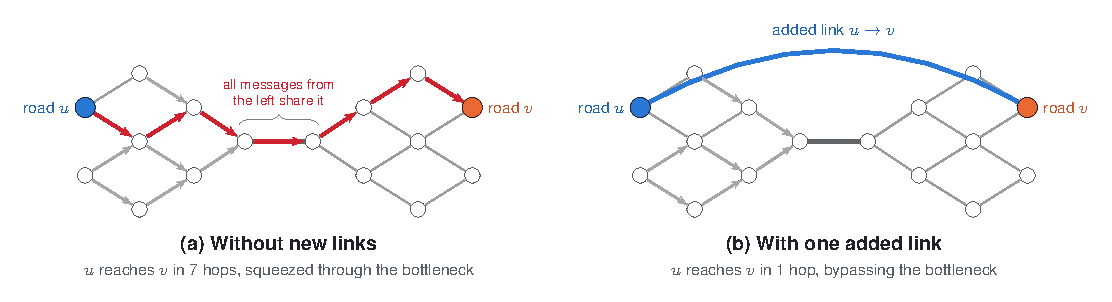
\includegraphics[width=0.78\textwidth]{figs/bottleneck_motivation.pdf}
\caption{\prev{Motivating example: an added link lets road $u$ reach road $v$ without passing through the bottleneck.}}
\label{fig:bottleneck}
\end{figure*}

\prev{Our motivation is the difficulty of hour-ahead forecasting under low-speed conditions. In our METR-LA baseline, mean absolute error (MAE) in the lowest speed band was more than twice the error across all readings. A slowdown at one sensor may provide early warning for another several hops away, suggesting that direct sensor links could make useful information more accessible. This leads to two questions: can a small number of added links improve low-speed forecasts, and does combining graph-connectivity information with predictive evidence help more than selecting links from predictive evidence alone? We distinguish these forecasting questions from the separate question of whether the models show evidence of reduced over-squashing.}

\prev{To investigate these questions, we add a budget of 25 directed links to the original road graph before training the forecaster. The initial greedy selector combines directional lead--lag correlation, \prev{which measures how strongly a slowdown at one sensor is followed by a slowdown at another a few minutes later}, with the reduction in total effective resistance produced by each addition. A follow-up compares two ridge-based selectors with the same final ranking procedure: Express Links shortlists weakly connected sources using pairwise effective resistance, whereas Forecast-only shortlists sources using predictive gain. The shortlisted links are ranked on a later block of training data. This predictive screen is related to the use of additional past information in Granger-style forecasting \cite{granger1969}, but is used here to select links rather than establish causal relationships.}

\prev{Our contributions are as follows.}
\begin{itemize}
\item \prev{We develop and evaluate a greedy selector that combines directional lead--lag correlation with total effective-resistance reduction, and compare it with six reference graphs, including a same-district control matched on lead--lag strength.}
\item \prev{We compare resistance-based and predictive shortlists within a common ridge-screening procedure on METR-LA and PEMS-BAY using Graph WaveNet, and evaluate the same frozen METR-LA graphs with DCRNN.}
\item \prev{We assess reliance on the selected sources using two input-replacement diagnostics, and evaluate changes to link number, distance, weight and allocation through validation-based tuning and a five-seed final comparison.}
\end{itemize}

\prev{On METR-LA, Forecast-only beat matched random links on all three seeds with both Graph WaveNet and DCRNN for 60-minute low-speed forecasts at the shared evaluation roads. The global virtual node achieved the lowest network-wide MAE in the six-way comparison.}

\prev{The rest of this report is organized as follows. Section~\ref{sec:related} reviews related work. Section~\ref{sec:methods} describes the forecasting task, the two link selectors and the control graphs. Section~\ref{sec:setup} gives the data, models and evaluation protocol, and Section~\ref{sec:results} reports the results. Section~\ref{sec:discussion} discusses what the results show, Section~\ref{sec:limitations} covers limitations and future work, and Section~\ref{sec:conclusion} concludes.}
